\documentclass[tikz,border=5pt]{standalone}
\usepackage[T1]{fontenc}
\usepackage{lmodern,amsmath,amssymb}
\usetikzlibrary{arrows.meta,calc,positioning,fit,backgrounds,shapes.geometric,matrix,decorations.pathreplacing,patterns}
\definecolor{ink}{gray}{0.08}
\definecolor{wash}{gray}{0.965}
\definecolor{soft}{gray}{0.45}
\tikzset{box/.style={draw=ink,line width=.65pt,fill=white,align=center,inner sep=4pt,outer sep=0pt,font=\small},flow/.style={draw=ink,line width=.65pt,-{Latex[length=1.8mm,width=1.3mm]},rounded corners=2pt},annotation/.style={font=\scriptsize,text=soft,align=center},groupbox/.style={draw=soft,dashed,line width=.45pt,fill=wash}}
\begin{document}
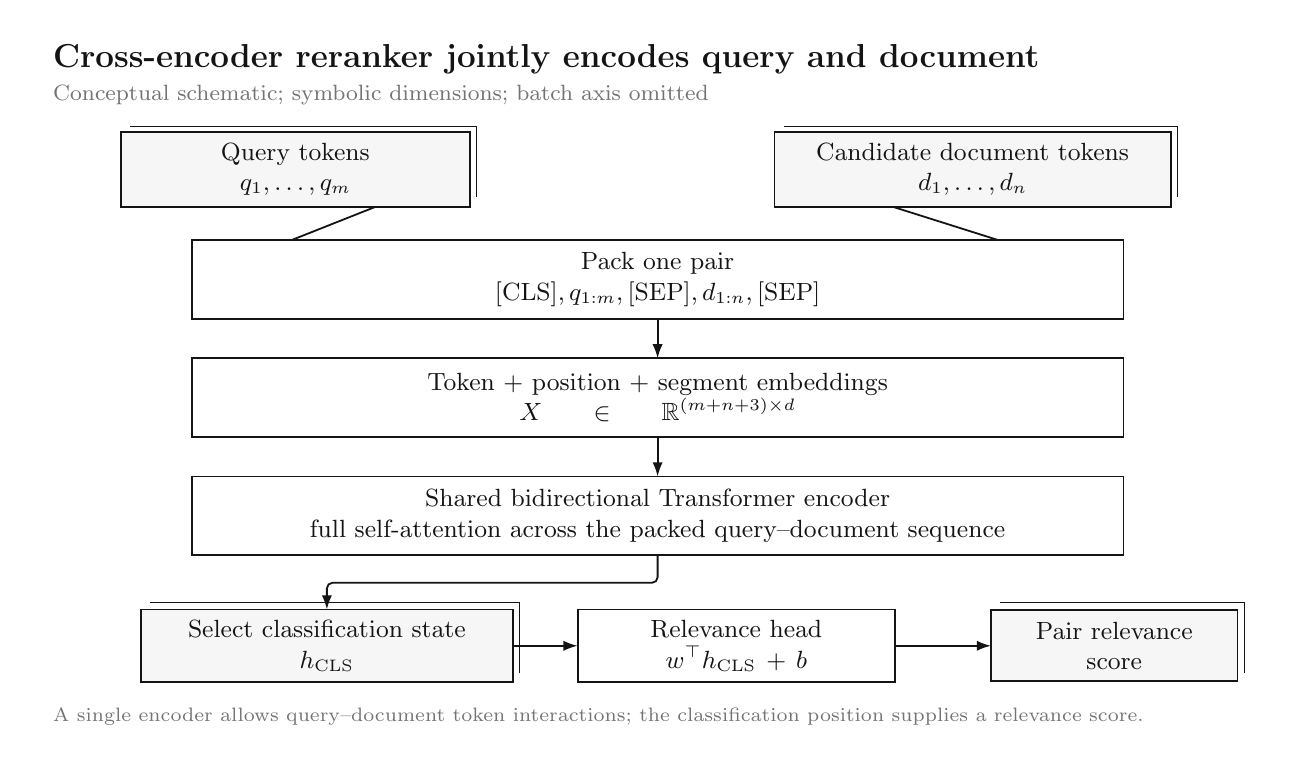
\begin{tikzpicture}[x=1cm,y=-1cm,font=\rmfamily,text=ink]

\path[use as bounding box] (0,0) rectangle (16,9);
\node[anchor=west,font=\large\bfseries] at (.2,.4) {Cross-encoder reranker jointly encodes query and document};
\node[anchor=west,font=\footnotesize,text=soft] at (.2,.85) {Conceptual schematic; symbolic dimensions; batch axis omitted};
\begin{pgfonlayer}{background}
\end{pgfonlayer}
\node[box,fill=wash,minimum width=4.4cm,minimum height=0.9cm,text width=4.15cm] (q) at (3.4,1.8) {Query tokens\\$q_1,\ldots,q_m$};
\draw[ink,line width=.4pt] (1.2999999999999998,1.25) -- (5.699999999999999,1.25) -- (5.699999999999999,2.15);
\node[box,fill=wash,minimum width=5cm,minimum height=0.9cm,text width=4.75cm] (d) at (12.0,1.8) {Candidate document tokens\\$d_1,\ldots,d_n$};
\draw[ink,line width=.4pt] (9.6,1.25) -- (14.6,1.25) -- (14.6,2.15);
\node[box,minimum width=11.8cm,minimum height=1.0cm,text width=11.55cm] (pack) at (8,3.2) {Pack one pair\\$[\mathrm{CLS}],q_{1:m},[\mathrm{SEP}],d_{1:n},[\mathrm{SEP}]$};
\node[box,minimum width=11.8cm,minimum height=1.0cm,text width=11.55cm] (embed) at (8,4.7) {Token $+$ position $+$ segment embeddings\\$X\in\mathbb{R}^{(m+n+3)\times d}$};
\node[box,minimum width=11.8cm,minimum height=1.0cm,text width=11.55cm] (enc) at (8,6.2) {Shared bidirectional Transformer encoder\\full self-attention across the packed query--document sequence};
\node[box,fill=wash,minimum width=4.7cm,minimum height=0.9cm,text width=4.45cm] (cls) at (3.8,7.85) {Select classification state\\$h_{\rm CLS}$};
\draw[ink,line width=.4pt] (1.5499999999999998,7.3) -- (6.25,7.3) -- (6.25,8.2);
\node[box,minimum width=4.0cm,minimum height=0.9cm,text width=3.75cm] (head) at (9,7.85) {Relevance head\\$w^\top h_{\rm CLS}+b$};
\node[box,fill=wash,minimum width=3.1cm,minimum height=0.9cm,text width=2.85cm] (score) at (13.8,7.85) {Pair relevance\\score};
\draw[ink,line width=.4pt] (12.35,7.3) -- (15.450000000000001,7.3) -- (15.450000000000001,8.2);
\begin{pgfonlayer}{background}
\draw[flow] (q.east) -- (pack.west);
\draw[flow] (d.west) -- (pack.east);
\draw[flow] (pack.south) -- (embed.north);
\draw[flow] (embed.south) -- (enc.north);
\draw[flow] (enc.south) -- (8,7.05) -- (3.8,7.05) -- (cls.north);
\draw[flow] (cls.east) -- (head.west);
\draw[flow] (head.east) -- (score.west);
\end{pgfonlayer}
\node[anchor=west,align=left,font=\scriptsize,text=soft,text width=15.6cm] at (.2,8.75) {A single encoder allows query--document token interactions; the classification position supplies a relevance score.};
\end{tikzpicture}
\end{document}
